\subsection{Machine Learning \& Hybrid Classification Pipeline}
\label{subsec:classification_pipeline}
The terminal stage of the pipeline architecture systematically shifts from abstract statistical geometry toward active, clinical interpretive reasoning. The fundamental design constraint—resolving both chaotic image matrices (scalograms) and highly abstracted dimensional features (PCA/Fuzzy logic outputs)—necessitates a split framework. Implemented across \texttt{pipeline/src/ML}, \texttt{pipeline/src/Fuzzy}, and the terminal \texttt{pipeline/src/interpreter} blocks, this tier unifies rigid deterministic probability logic alongside biologically mapped soft-computing boundaries \cite{jang1993anfis, oh2019deep}.

\begin{figure}[htpb]
    \centering
    \resizebox{\textwidth}{!}{
    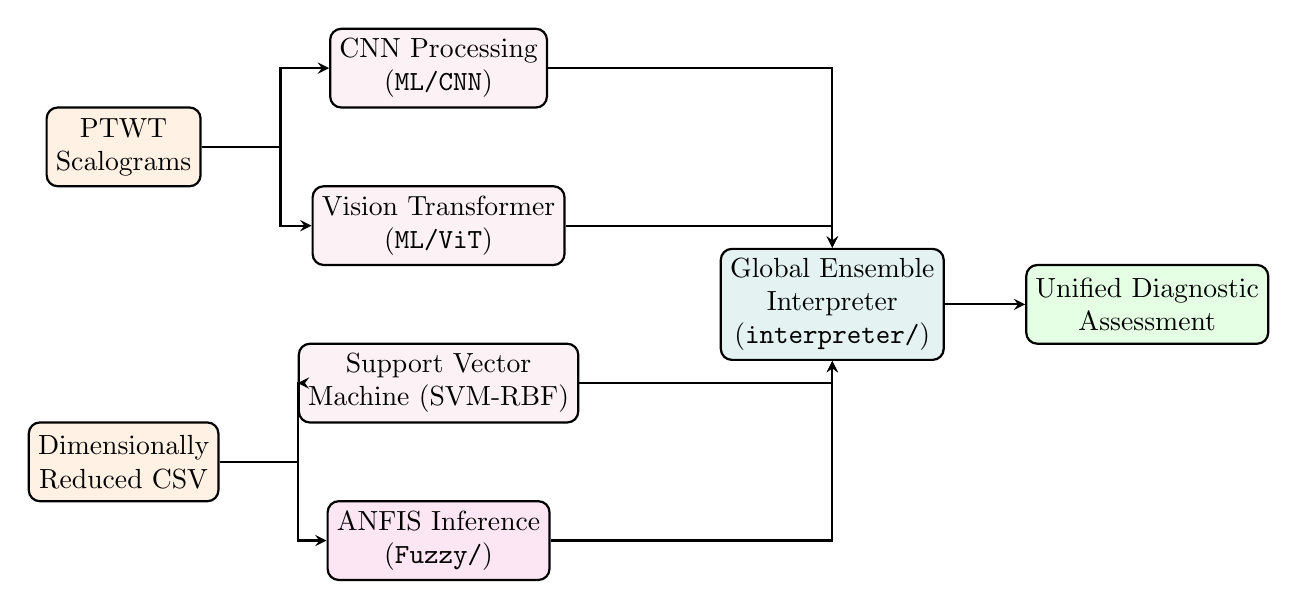
\begin{tikzpicture}[
        box/.style={draw, rectangle, rounded corners, align=center, minimum height=1cm, fill=purple!5, thick},
        arrow/.style={->, thick, -stealth}
    ]
        % Inputs
        \node[box, fill=orange!10] (img) at (0, 2) {PTWT \\ Scalograms};
        \node[box, fill=orange!10] (csv) at (0, -2) {Dimensionally \\ Reduced CSV};

        % Deep Learning
        \node[box] (cnn) at (4, 3) {CNN Processing \\ (\texttt{ML/CNN})};
        \node[box] (vit) at (4, 1) {Vision Transformer \\ (\texttt{ML/ViT})};

        % Traditional / Fuzzy
        \node[box] (trad) at (4, -1) {Support Vector \\ Machine (SVM-RBF)};
        \node[box, fill=magenta!10] (fuzzy) at (4, -3) {ANFIS Inference \\ (\texttt{Fuzzy/})};

        % Ensamble
        \node[box, fill=teal!10] (ensemble) at (9, 0) {Global Ensemble \\ Interpreter \\ (\texttt{interpreter/})};
        
        \node[box, fill=green!10] (final) at (13, 0) {Unified Diagnostic \\ Assessment};

        % Paths
        \draw[arrow] (img.east) -- ++(1,0) |- (cnn.west);
        \draw[arrow] (img.east) -- ++(1,0) |- (vit.west);
        
        \draw[arrow] (csv.east) -- ++(1,0) |- (trad.west);
        \draw[arrow] (csv.east) -- ++(1,0) |- (fuzzy.west);

        \draw[arrow] (cnn.east) -| (ensemble.north);
        \draw[arrow] (vit.east) -| (ensemble.north);
        \draw[arrow] (trad.east) -| (ensemble.south);
        \draw[arrow] (fuzzy.east) -| (ensemble.south);

        \draw[arrow] (ensemble.east) -- (final.west);

    \end{tikzpicture}
    }
    \caption{Structure of the comprehensive machine learning interpretation sequence bridging complex visual transformers and rigid fuzzy decision boundaries via localized ensemble voting.}
    \label{fig:classification_process}
\end{figure}

\subsubsection{Visual Deep Learning Architectures (ML Stack)}
Capitalizing entirely on the rich time-frequency representations encoded within PyTorch-generated Continuous Wavelet Scalograms, the architecture instantiates rigid image-parsing algorithms inside the \texttt{ML} sub-directories.

\paragraph{Convolutional and Attention-Driven Networks}
Traditional classification handles basic geometric clustering cleanly; however, extracting distributed, high-latency structural abnormalities associated with 40-Hz gamma disruptions requires deeper mechanisms \cite{dosovitskiy2021vit}. The primary sub-modules deploy custom CNN (Convolutional Neural Network) stacks and, more critically, state-of-the-art \textbf{Vision Transformers (ViT)}. 
While CNNs perform localized feature extraction via bounded Gaussian kernels $K \ast S(a,b)$, the Vision Transformer actively fragments the raw input scalogram image $S$ into linear patch arrays. Using multi-headed self-attention parameters directly on chronological signal-patch blocks allows the ViT core to natively understand generalized, long-range dependencies—i.e., mapping a low-frequency artifact occurring globally to a highly specific, localized gamma burst disruption occurring significantly later.

\subsubsection{Fuzzy Decision and Neural Soft-Voting}
Parallel to the black-box mapping generated within deep networks, the pipeline requires transparent localized evidence. Implemented via \texttt{membership.py} in the \texttt{Fuzzy/} directories, the framework introduces explicit degrees of uncertainty mapping structural cognitive decline.

Given the non-stationarity of the base EEG (and natural physiological drift due to subject anatomy), rigid boolean states invariably misdiagnose edge boundaries. The classification sub-engine integrates an Adaptive Neuro-Fuzzy Inference System (ANFIS), constructing functional trapezoidal/Gaussian envelopes specifically optimized using FCM (Fuzzy C-Means). 
The inference outputs are continuously valued, resolving arbitrary risk probabilities based purely on fuzzy weight activation rather than strict probability thresholds. This essentially permits algorithms to register ``Moderate to High Confidence of Atrophy'' explicitly bound to fuzzy feature drift patterns (like Katz Fractional mapping changes), vastly enhancing clinical transparency. 

\subsubsection{The Global Ensemble Interpreter}
Categorical deep-learning matrices and soft mathematical rules naturally conflict. Therefore, localized decision outcomes are fed continuously into \texttt{ensemble.py} nested inside the \texttt{interpreter/} module. 
The interpreter logic acts not merely as an averaging switch, but rather functions dynamically through weighted soft-voting rules constrained by informational entropy. For example, if continuous artifact clipping causes high-entropy (ambiguous) visual patterns leading the ViT map to exhibit diagnostic uncertainty, the interpreter script heavily shifts probabilistic weight directly onto the reduced-feature SVM and ANFIS mappings. This cross-verification loop severely limits false-positive risk probabilities stemming dynamically out of pure technical noise and perfectly satisfies proof-of-concept demands for structurally resilient neuro-computation \cite{ribeiro2016lime}.